\documentclass[12pt]{article}

\usepackage{fancyhdr}
\usepackage{geometry}
\usepackage{graphicx}

%Page Margins and Size
\geometry{
a4paper,
total={170mm,257mm},
left=20mm,
top=30mm,
bottom=30mm,
}
 

%Headers and Footers 
\pagestyle{fancy}
\fancyhf{}
\lhead{User Manual}
\cfoot{\thepage}
 
\begin{document}

	\begin{titlepage}		%cover page of document

		{\Huge UG-17 Rover Controller}

		\vspace{0.5cm}

		{\Huge User Manual}


	\end{titlepage}

	\clearpage


	\tableofcontents
	\clearpage


	

	\section{Introduction}
The user interface is a control panel displaying the map of the area the Rover is exploring, and updating all map features found by the Rover on it in real time. It has various options to directly control the Rover’s movements, such as movement keys (up, down, left and right), return to landing site button, emergency button, and etc. It also includes options to import, export and functionalities to customise the Rover map. The main components which form this subsystem are illustrated below under the main section.
	
	\section{GUI and Rover startup}
To initialise the rover and GUI such that a connection can be established, the StartRover.jar program must first be executed on the rover. This will create the server which the GUI will connect to. Once the rover has beep (indicates server is ready to connect to), the GUI can be started and will automatically connect to the rover through a BlueTooth access point. 
	
	\section{Main Sections}
		\begin{center}
		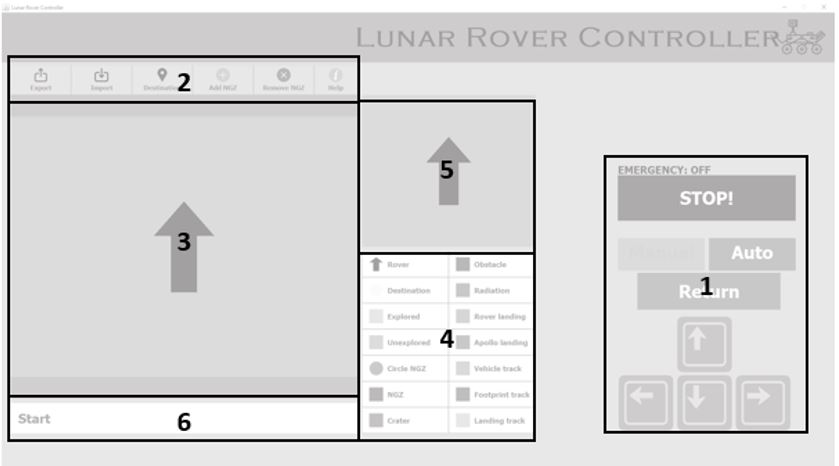
\includegraphics[scale=1]{RoverController.jpg}
		\end{center}		
	\subsection{Main Control Panel}
This is where the user issues commands that directly affect the Rover’s behaviour. The user can let the Rover survey the area by itself with predefined algorithms in Auto Mode, or switch to Manual Mode to control the Rover directly with the arrow keys. There’s also an emergency button to freeze the Rover in case its self protection program didn’t suffice.
	\subsubsection{Option available in both Auto and Manual mode}	
		\begin{center}		
		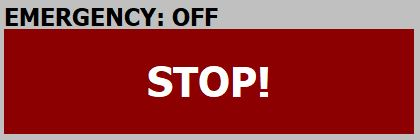
\includegraphics[scale = 1]{Emergency.jpg}
		\end{center}
Emergency button: Clicking it once will trigger the Emergency Mode, which will freeze the bot where it is, and it will not perform any action until the Emergency Mode is disengaged by a double click (two clicks within 1.5 seconds).	
	
	\subsubsection{Option available in Auto mode only}
		\begin{center}
		
\includegraphics[scale = 1]{Manual.jpg}	
		\end{center}	
Manual option: It will set the Rover into Manual Mode, which is the default mode, stopping current actions and erasing all planned future actions, including the destinations set for the Rover to travel to.
\\*
		\begin{center}
		
\includegraphics[scale = 1]{Return.jpg}
		\end{center}
Return option: It will command the Rover to go back to the starting point in the fashion of going after a user set goal point. It will not stop until the user switches to Manual Mode.
	
	\subsubsection{Option available in Manual mode only}
		\begin{center}
		
\includegraphics[scale = 1]{Auto.jpg}
		\end{center}	
Auto option: It will set the Rover into Auto Mode. Under Auto Mode, the Rover will automatically navigate to user defined goal points if there are any, else it will go after unexplored area in the map to survey the area. When all safe area (non-NGZ) are explored, it will return to the landing site in the fashion that it goes to a user designated goal point.
\\*
		\begin{center}
		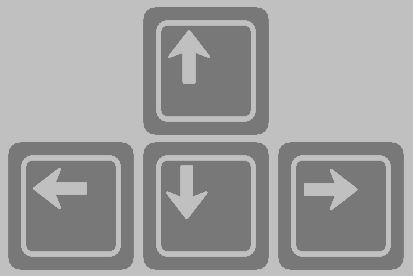
\includegraphics[scale = 1]{Arrows.jpg}
		\end{center}	
Arrow keys: They issue orders to let the Rover move in the direction relative to the direction the Rover’s currently facing. So when the Rover is facing right on the Rover Map, pressing up arrow will make it go forward to the right. There can be only one active key at a time.
\\*
\\*
\textit{Note: There is also a toolbar operation available in Auto Mode only, which will be explained in the next section.}

		
	\subsection{Toolbar}
		\begin{center}
		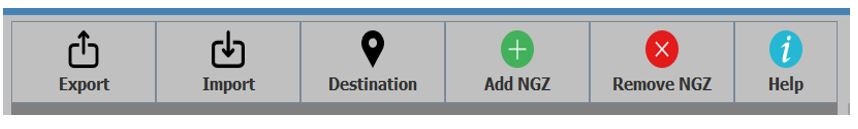
\includegraphics[scale=1]{ToolBar.jpg}
		\end{center}	
The toolbar consists of 6 options: Export, Import, Destination, Add NGZ, Remove NGZ, and Help. Only one of the toolbar functionalities can be chosen at a time. The Destination, Add and Remove NGZ function can be disengaged by clicking the button again or by selecting the other toolbar options. The options of Destination is available in Auto Mode only.

	\subsubsection{Export/Import Buttons}
Export button: used to save the current map data into an .XML file on the user’s computer. The user can either save on a new .XML file or override on a .XML file. 
\\*
\\*
Import button: used to load in the data of an existing map .XML file to the software’s Rover map. This function will override the current map data.
\\*
\\*
Clicking the Export/Import button opens up a file explorer that helps you to navigate through the folders. The diagram below explains the functionalities in a file explorer.
		\begin{center}
		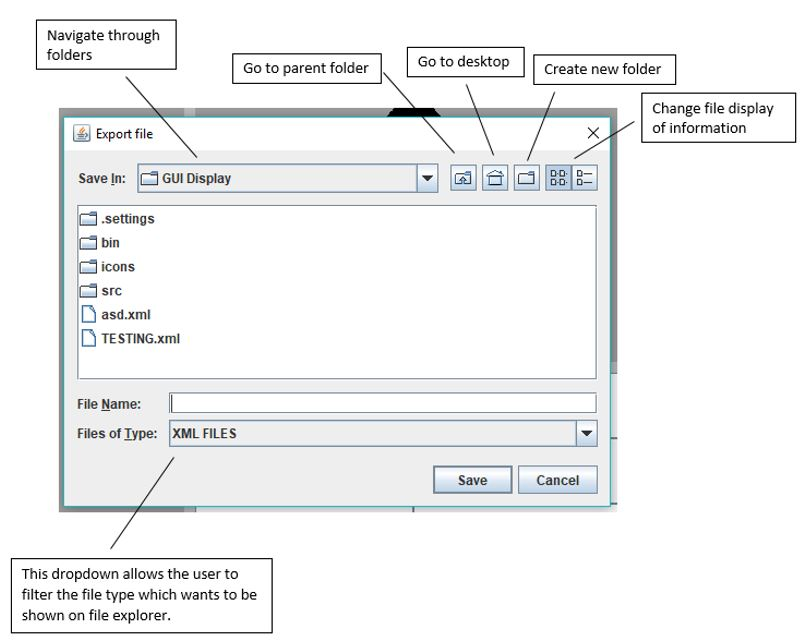
\includegraphics[scale=1]{FileExplorer.jpg}
		\end{center}
	
	\subsubsection{Destination Button}
The Destination button will allow the user to set the rover’s destinations by clicking on the Rover Map. The function will only work when the Rover is in Auto Mode and will mark up to three locations at a time. When a destination has been set the Rover will navigate to the location in the order in which they were set. When Manual Mode is engaged the set destinations will be removed from memory and will not carry over when switching back to Auto Mode. When a new destination is set and there were already three, the earliest one will be removed before the new one is added. All destination points will be removed when the user switches to Manual Mode. Destination points  won’t be saved when exporting maps.	
		\begin{center}
		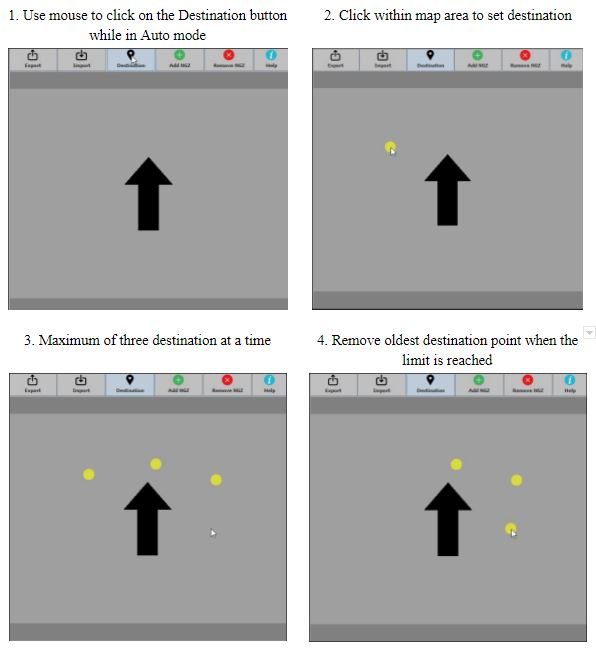
\includegraphics[scale=1.1]{Destination.jpg}
		\end{center}
	
	\subsubsection{Add/Remove NGZ Buttons}
Add NGZ button: allows the user to draw NGZ areas onto the Rover Map. To Draw NGZ areas the user will need to use the mouse and proceed to left click and drag the mouse around to indicate the desired shape, upon release a filled in area indicating the NGZ will be generated. Drawing is limited to the map area indicated by a lighter grey colour and will draw along the edge when the mouse is moved out of this area.
		\begin{center}
		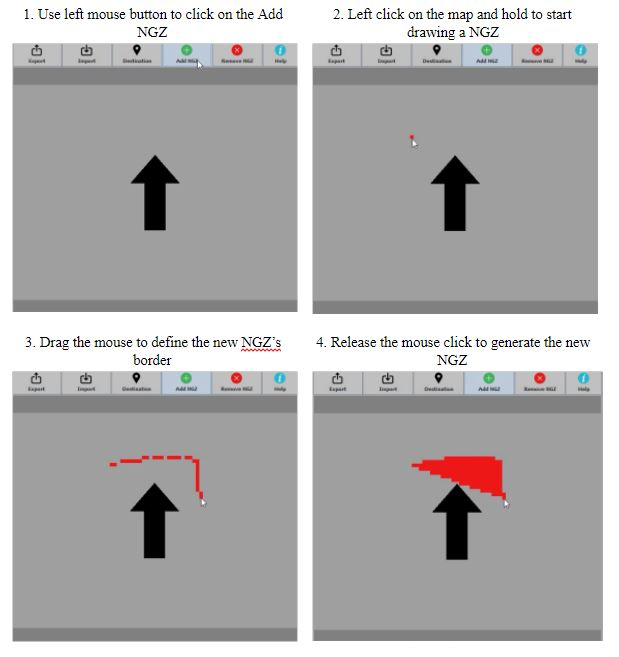
\includegraphics[scale=1.1]{AddNGZ.jpg}
		\end{center}
Remove NGZ button: allows the user to remove user drawn NGZs on the Rover Map. To remove the NGZ the user will needs to do a left click within an NGZ, holding down and dragging the left mouse button will also work and is recommended for NGZ lines. 
	
	\subsubsection{Help Button}
Clicking the Help button opens up the user manual (this file). The user manual is a technical document that provides explanations on how to operate the Rover controller and each of the elements’ functionalities.
		
	\subsection{Rover Map}
		\begin{center}
		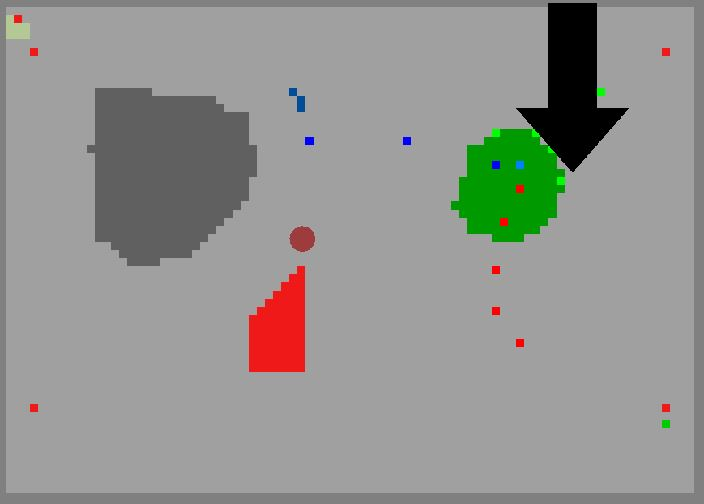
\includegraphics[scale=0.7]{RoverMap.jpg}
		\end{center}
The Rover Map allows the user to graphically view the Rover's map data and provides several additional  functionalities. The default setting allows the user to use mouse to click and drag the map around with the left mouse button. Panning of the map is disabled when either the Destination, Add NGZ and Remove NGZ buttons have been engaged. Using the add and subtract buttons on the numpad will allow the user to zoom in and out respectively.
	
	\subsection{Legend}
		\begin{center}
		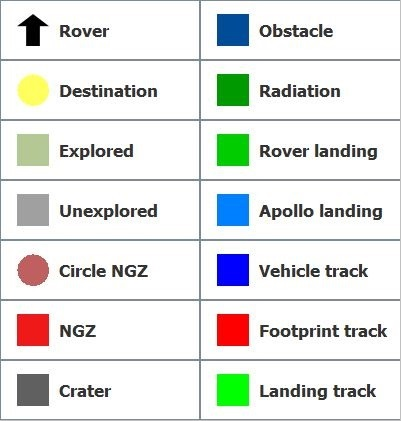
\includegraphics[scale=1]{Legend.jpg}
		\end{center}
There’s a legend panel under the Mini Map, on the right of Status Bar. The colors of all items shown on the Rover Map are configurable. After clicking on one slot, a color selection window will pop up:
		\begin{center}
		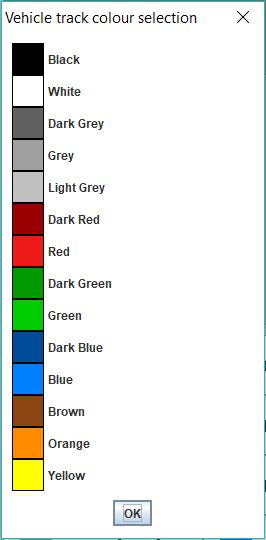
\includegraphics[scale=1]{ColourSelection.jpg}
		\end{center}
The user can then click on the preferred color and click on OK, and the corresponding element on the map will be updated to the selected color. Only the track colours will be saved to the .XML file.
		
	\subsection{Mini Map}
		\begin{center}
		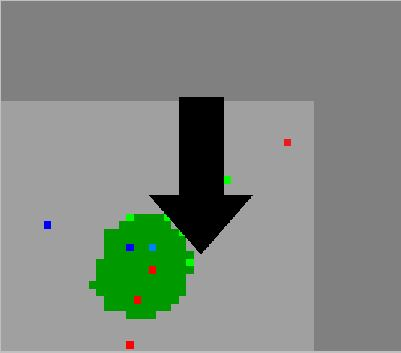
\includegraphics[scale=1]{MiniMap.jpg}
		\end{center}
The Mini Map displays the map with the Rover icon being zoomed in and centrally fixed. The elements presented on the Rover Map are also visible on the Mini Map; however, the Mini Map cannot be used to add map functions. Its intended purpose is to allow the user to keep track of the Rover and its surroundings, while Rover Map has functions, such as zooming and panning, that  potentially allows the user to lose track of the Rover.
		
	\subsection{Status Bar}
		\begin{center}
		
\includegraphics[scale=1]{StatusBar.jpg}
		\end{center}
The status bar is located under the rover map. It  presents information on the Rover’s latest state, actions, or map element discoveries.
\\*
		\begin{center}
		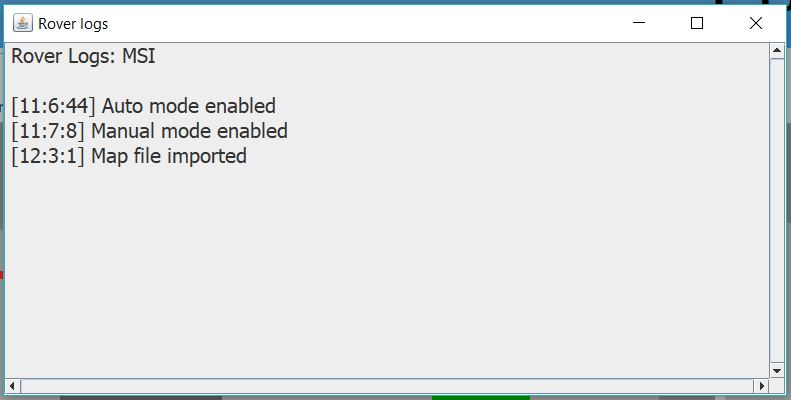
\includegraphics[scale=1]{RoverLog.jpg}
		\end{center}
The status bar can be clicked to open up the Rover Log. The rover log provides a list of real-time information of  the Rover’s state, actions, and discoveries ever since the run time of the program. Along with the Rover’s information, it also shows the timing of when the event have occurred. 
		
	
	\section{Abbreviation}
GUI: Graphical User Interface
\\*
NGZ: No go zone, it’s defined as an area that the Rover shouldn’t go into.
		
\end{document}